\begin{exo}
	Dans l'arbre ci-dessous, exprimer chacune des pondérations comme une probabilité (par ex. $0,65 = P_{A}\left(\overline{B}\right)$)

	\begin{center}
		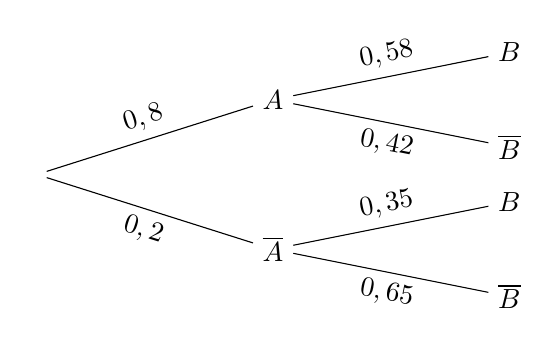
\begin{tikzpicture}[grow=right,sloped, level distance=3cm,
				level 1/.style={sibling distance=1.9cm},
				level 2/.style={sibling distance=1.2cm}]
			\node {}
			child {node {$\overline{A}$}
					child {node {$\overline{B}$} edge from parent node[below] {$0,65$}}
					child {node {$B$} edge from parent node[above] {$0,35$}}
					edge from parent node[below] {$0,2$}
				}
			child {node {$A$}
					child {node {$\overline{B}$} edge from parent node[below] {$0,42$}}
					child {node {$B$} edge from parent node[above] {$0,58$}}
					edge from parent node[above] {$0,8$}
				};
		\end{tikzpicture}
	\end{center}
\end{exo}
